\chapter{Implementazione delle tecnologie}\label{capitolo-4}
In questo capitolo ci occuperemo di applicare le tecnologie trattate nel capitolo 4, andando a sviluppare la web app "Postit-app", nella quale sarà possibile effettuare il login con il proprio account e creare, aggiornare ed eliminare delle note (postit) nella home page del sito. Ogni postit è costituito da un titolo e una descrizione.

\section{Implementazione back-end}


\subsection{Database}
Per prima cosa mi sono occupato dell'implementazione del database, e per fare ciò l'ho creato utilizzando docker eseguendo il seguente comando:
\\
\begin{lstlisting}[language=xml,basicstyle=\small, caption={Creazione del DB "postit-app-db"}, captionpos=b]
docker run --name postit-app-db ^
 -e POSTGRES_USER=utente ^
 -e POSTGRES_DB=postit-app-db ^
 -e POSTGRES_PASSWORD=password ^
 -e PGDATA=/var/lib/postgresql/data/postitData ^
 -p 5434:5432 ^
 -v C:\Docker_Data:/var/lib/postgresql/data ^
 postgres:14.1-alpine
\end{lstlisting}

Successivamente al fine di gestire i dati nel db e creare le diverse tabelle necessarie alla web app, ho utilizzato DBeaver, un'applicazione software client SQL e uno strumento di amministrazione di database.
Una volta effettuata la connessione al DB ho creato diverse tabelle:
\begin{itemize}
    \item users
    \item roles
    \item postit
\end{itemize}
\newpage
\subsubsection{Tabella users}
All'interno della tabella users ho inserito gli utenti con le loro rispettive password criptate.
\begin{lstlisting}[language=sql,basicstyle=\small, caption={Creazione tabella users}, captionpos=b]
CREATE TABLE users (
    user_id varchar(50) not null primary key,
    pw char(68) not null,
    active int not null);
\end{lstlisting}
\begin{lstlisting}[language=sql,basicstyle=\small, caption={Inserimento dati degli utenti in users}, captionpos=b]
INSERT INTO users VALUES
    ('john','{bcrypt}$2a$10$qeS0HEh7urweMojsnwNAR.vcXJeXR1UcMRZ2WcGQl9YeuspUdgF.q',1),
    ('mary','{bcrypt}$2a$10$qeS0HEh7urweMojsnwNAR.vcXJeXR1UcMRZ2WcGQl9YeuspUdgF.q',1),
    ('susan','{bcrypt}$2a$10$qeS0HEh7urweMojsnwNAR.vcXJeXR1UcMRZ2WcGQl9YeuspUdgF.q',1);
\end{lstlisting}

\subsubsection{Tabella roles}
Al fine di gestire l'accesso a determinate pagine della web app, ad ogni utente è associato un ruolo.
\begin{lstlisting}[language=sql,basicstyle=\small, caption={Creazione tabella roles}, captionpos=b]
CREATE TABLE roles (
    user_id varchar(50) references users(user_id),
    ruolo varchar(50) not null);
\end{lstlisting}
\begin{lstlisting}[language=sql,basicstyle=\small, caption={Inserimento dei ruoli nella tabella}, captionpos=b]
INSERT INTO roles VALUES
    ('john','ROLE_EMPLOYEE'),
    ('mary','ROLE_EMPLOYEE'),
    ('susan','ROLE_EMPLOYEE');
\end{lstlisting}

\subsubsection{Sequence per gestione dell'id}
Al fine di garantire un incremento dell'id numerico di ogni postit ho creato una sequence, che ho poi utilizzato nella creazione della tabella postit.
\begin{lstlisting}[language=sql,basicstyle=\small, caption={Creazione della sequence per l'id del postit}, captionpos=b]
create sequence seq_postit
increment by 1
start with 1
minvalue 1
no maxvalue;
\end{lstlisting}

\subsubsection{Tabella postit}
All'interno della tabella postit vengono salvati tutti i dati delle note e l'utente che ha creato queste ultime.
\begin{lstlisting}[language=sql,basicstyle=\small, caption={Creazione tabella postit}, captionpos=b]
CREATE TABLE postit (
    id bigint primary key default nextval ('seq_postit'),
    body varchar,
    title varchar,
    "timestamp" timestamp with time zone default current_timestamp,
    user_id varchar(50) references users(user_id));
\end{lstlisting}

\subsection{Classe Postit}
Al fine di far si che i record salvati all'interno della tabella postit, possano essere trasformati in un oggetto Java ho creato la classe Postit e per garantire questa comunicazione ho utilizzato diverse annotation:
\begin{itemize}
    \item @Entity: per far si che un oggetto Java possa interfacciarsi con il db;
    \item @Table: per associare la classe Postit alla tabella postit salvata nel db;
    \item @Column: per associare la colonna della tabella alla variabile della classe;
    \item @Id: per indicare che la variabile è un id;
    \item @SequenceGenerator: per associare la sequence del db alla variabile della classe, garantendo l'incremento automatico.
\end{itemize}
\begin{lstlisting}[language=Java,basicstyle=\tiny, caption={Classe PostIt.java}, captionpos=b]
@Entity
@Table(name = "postit")
@Getter
@Setter
@NoArgsConstructor
@AllArgsConstructor
@Builder
public class PostIt {

    @Id
    @GeneratedValue(strategy = GenerationType.SEQUENCE, generator = "seq_postit")
    @SequenceGenerator(name = "seq_postit", sequenceName = "seq_postit", allocationSize = 1)
    @Column(name = "id")
    private Long id;

    @Column(name = "body")
    private String body;

    @Column(name = "title")
    private String title;

    @Column(name = "timestamp")
    @UpdateTimestamp
    private LocalDateTime timestamp;

    @Column(name = "user_id")
    private String userId;

}

\end{lstlisting}
\newpage
\subsection{Interfaccia e classe PostitService}
In mezzo alla comunicazione tra template, controller e repository vi è la classe Service la quale si occupa di chiamare i metodi della classe repository dopo l'esecuzione di un metodo del controller.
Prima di implementare la classe PostitService ho definito un'interfaccia con al suo interno tutti i metodi utilizzati.\\
\begin{lstlisting}[language=Java,basicstyle=\small, caption={Interfaccia PostitService.java}, captionpos=b]
public interface PostitService {

    public List<PostIt> findByUser_id(String userId);
    
    public void save(PostIt thePostit);
    
    public void deleteById(Long id);

}
\end{lstlisting}
Successivamente ho implementato la classe PostitService e ho utilizzato l'annotation @Service per indicare che la classe fa da service.
All'interno di questa classe come attributo vi è l'oggetto che ci permette di riferirci alla repository e quindi a comunicare con il DB.\\
Il metodo findByUser\_id permette di cercare nel database tutti i postit che hanno come user id il valore passato come parametro, restituendo una lista di postit.\\
Il metodo save viene utilizzato per salvare un nuovo postit oppure uno modificato.\\
Il metodo deleteById permette di eliminare un postit specificando il suo id.
\begin{lstlisting}[language=Java,basicstyle=\small, caption={Classe PostitServiceImpl.java}, captionpos=b]
@Service
public class PostitServiceImpl implements PostitService {

    @Autowired
    private PostitRepository repo;

    @Override
    public List<PostIt> findByUser_id(String userId) {
        return repo.findByUserId(userId);
    }

    @Override
    public void save(PostIt thePostit) {
        repo.save(thePostit);
    }

    @Override
    public void deleteById(Long id) {
        repo.deleteById(id);
    }
}
\end{lstlisting}
\newpage
\subsection{Interfaccia PostitRepository}
L'interfaccia PostitRepository si occupa di interfacciarsi con il DB eseguendo le diverse operazioni richieste da parte del service. Per indicare che un'interfaccia o una classe è una repository ho usato l'annotation @Repository.
In Spring Boot, grazie a JPA, è possibile estendere questa interfaccia con la classe JpaRepository<PostIt, Long> la quale fornisce automaticamente tutte le operazioni CRUD, senza la necessità di dover scrivere metodi che le implementino. In particolar modo tra le parentesi angolate come primo attributo va inserita la classe che voglio utilizzare e come secondo attributo specifico il tipo dell'id della classe utilizzata, ovvero la classe PostIt.\\
\begin{lstlisting}[language=Java,basicstyle=\small, caption={Interfaccia PostitRepository che estende JpaRepository}, captionpos=b]
@Repository
public interface PostitRepository extends JpaRepository<PostIt,Long> {

    List<PostIt> findByUserId(String nome);

}
\end{lstlisting}
\subsection{Login controller}
Al fine di gestire le richieste da parte del browser per effettuare il login, ho creato la classe LoginController, nella quale ho il metodo showMyLoginPage, che una volta ricevuta la richiesta permette la visualizzazione della pagina di login.\\
Il metodo accessDenied visualizza la pagina di accesso negato, nel caso in cui un utente non possedesse i permessi per visualizzare la homepage.

In questa classe ho usato due annotation:
\begin{itemize}
    \item @Controller: per indicare che la classe è un controller.
    \item @GetMapping: per gestire la richiesta del browser. Ad esempio se nell'url è presente l'endpoint "/login", il controller si occuperà di mostrare la pagina di login eseguendo il metodo showMyLoginPage.
\end{itemize}
\newpage
\begin{lstlisting}[language=Java,basicstyle=\small, caption={Login controller}, captionpos=b]
@Controller
public class LoginController {

    @GetMapping("/login")
    public String showMyLoginPage() {

        return "login-page";
    }

    @GetMapping("/access-denied")
    public String accessDenied() {

        return "access-denied";
    }
    
}
\end{lstlisting}
\subsection{Postit controller}
La classe PostItController si occupa di gestire tutte le richieste della homepage. Nello specifico si occupa di garantire il corretto funzionamento delle funzionalità CRUD (Create, Read, Update, Delete).
Inoltre in ogni metodo viene utilizzato il PostitService, che permette di comunicare con l'interfaccia PostitRepository, che a sua volta comunica con il db.

All'interno di questa classe è possibile trovare tre metodi:
\begin{itemize}
    \item getPersonalPostits: permette di recuperare tutti i postit dell'utente corrente, inserendoli all'interno del model il quale verrà utilizzato all'interno della pagina html per visualizzare i postit.
    \item addPostit: permette di gestire la richiesta di creazione e modifica di un postit.
    \item deleteById: permette di gestire la richiesta di eliminazione di un postit.
\end{itemize}
\newpage
\begin{lstlisting}[language=Java,basicstyle=\small, caption={Postit Controller}, captionpos=b]
@Controller
@RequestMapping("/postit")
@RequiredArgsConstructor
public class PostItController {

    private final PostitService service;

    @GetMapping("/all")
    public String getPersonalPostits(Authentication authentication, Model theModel) {
        List<PostIt> personalPostits = service.findByUser_id(authentication.getName());
        PostIt p = new PostIt();
        theModel.addAttribute("postits", personalPostits);
        theModel.addAttribute("postitSingolo", p);

        return "postit-home";
    }

    @PostMapping("/add/single")
    public String addPostit(@ModelAttribute("postit") PostIt thePostit, Authentication authentication) {
        thePostit.setUserId(authentication.getName());
        service.save(thePostit);

        return "redirect:/postit/all";
    }

    @GetMapping("/delete/single")
    public String deleteById(@RequestParam("postitId") Long theId) {
        service.deleteById(theId);

        return "redirect:/postit/all";
    }

}
\end{lstlisting}
\newpage
\subsection{Configurazione login}
Per la gestione del login ho utilizzato Spring Security e ho creato una classe di configurazione al fine di configurare la corretta autenticazione di un utente.\\
Per indicare che la classe si tratta di una configurazione ho usato l'annotation @Configuration.

In questa classe sono presenti due metodi:
\begin{itemize}
    \item userDetailsManager: si occupa di gestire gli utenti all'interno del database per recuperare l'id dell'utente, la password e il ruolo associato, al fine di garantire una corretta autenticazione dell'utente.
    \item filterChain: si occupa di gestire gli accessi alle pagine statiche e template a seconda del ruolo associato. Inoltre viene gestito il login in modo tale che ad un utente, dopo essersi autenticato, venga visualizzata la homepage. Oltre al login vengono gestite le eccezioni e il logout.
    
    Nel nostro caso, un utente a cui è associato il ruolo di "EMPLOYEE" può visualizzare la homepage e accedere a tutte le funzionalità della web app. Nel caso un utente avesse un ruolo diverso da "EMPLOYEE", verrebbe mandato alla pagina di accesso negato.
\end{itemize}
\begin{lstlisting}[language=Java,basicstyle=\tiny, caption={Classe SecurityConfig.java}, captionpos=b]
@Configuration
public class SecurityConfig {

    @Bean
    public UserDetailsManager userDetailsManager(DataSource dataSource) {

        JdbcUserDetailsManager jdbcUserDetailsManager = new JdbcUserDetailsManager(dataSource);

        jdbcUserDetailsManager.setUsersByUsernameQuery(
                "SELECT user_id, pw, active FROM users WHERE user_id=?");

        jdbcUserDetailsManager.setAuthoritiesByUsernameQuery(
                "SELECT user_id, ruolo FROM roles WHERE user_id=?");

        return jdbcUserDetailsManager;
    }

    @Bean
    public SecurityFilterChain filterChain(HttpSecurity http) throws Exception {

        http.authorizeHttpRequests(configurer ->
                        configurer
                                .requestMatchers(PathRequest.toStaticResources().atCommonLocations()).permitAll()
                                .requestMatchers("/login").permitAll()
                                .requestMatchers("/error").permitAll()
                                .requestMatchers("/postit/**").hasAnyRole("EMPLOYEE")
                                .anyRequest().authenticated()
                )
                .formLogin(form ->
                        form
                                .loginPage("/login")
                                .defaultSuccessUrl("/postit/all")
                                .loginProcessingUrl("/authenticateTheUser")
                                .permitAll()
                )
                .logout(LogoutConfigurer::permitAll

                )
                .exceptionHandling(configurer ->
                        configurer.accessDeniedPage("/access-denied")
                );

        return http.build();
    }


}
\end{lstlisting}
\newpage
\section{Implementazione front-end}
\subsection{Pagina di login}
All'interno della login-page.html è presente un form in cui l'utente può inserire l'username e la password per autenticarsi.
Se le credenziali di accesso sono corrette spring security si occuperà di mandare l'utente alla homepage. In caso contrario viene visualizzato un messaggio di errore.
\begin{lstlisting}[language=html,basicstyle=\tiny, caption={login-page.html}, captionpos=b]
<!DOCTYPE html>
<html lang="en" xmlns:th="http://www.thymeleaf.org">
  <head>
    <meta charset="UTF-8" />
    <meta name="viewport" content="width=device-width, initial-scale=1.0" />
    <link
      rel="stylesheet"
      href="https://cdnjs.cloudflare.com/ajax/libs/font-awesome/6.4.2/css/all.min.css"
    />
    <link th:href="@{/css/login.css}" type="text/css" rel="stylesheet" />

    <title>Login Page</title>
  </head>

  <body>
    <div class="container1" id="container">
      <div class="form-container sign-in">
        <form action="#" th:action="@{/authenticateTheUser}" method="POST">
          <h1>Sign In</h1>

          <div>
            <!-- Check for login error -->
            <div th:if="${param.error}">
              <div>
                <p class="invalid-username">Invalid username or password.</p>
              </div>
            </div>

            <div th:if="${param.logout}">
              <div class="alert alert-success col-xs-offset-1 col-xs-10">
                <p class="logout">You have been logged out.</p>
              </div>
            </div>
          </div>

          <input type="text" name="username" placeholder="Username" />
          <input type="password" name="password" placeholder="Password" />
          <button>Sign In</button>
        </form>
      </div>
      <div class="toggle-container">
        <div class="toggle">
          <div class="toggle-panel toggle-right">
            <h1>Welcome to the Postit App</h1>
            <p>Sign In to se your personal postits!</p>
          </div>
        </div>
      </div>
    </div>
  </body>
</html>

\end{lstlisting}
\newpage
\subsection{Homepage}
Nella pagina postit-home.html è presente una navbar in cui viene visualizzato il nome dell'utente e il suo ruolo. Inoltre sono presenti i bottoni che permettono di creare un nuovo postit ed effettuare il logout.
Al di sotto della navbar vengono visualizzati i postit, i quali hanno un titolo, una descrizione e i bottoni che permettono di modificare o eliminare il postit selezionato.
I postit vengono visualizzati grazie all'utilizzo di un foreach, il quale scorre la lista di postit creati dall'utente e per ognuno crea una card nella quale vengono inseriti i corrispettivi dati.
La lista di postit creati dall'utente viene recuperata grazie all'utilizzo del contenitore model di Thymeleaf.
\begin{lstlisting}[language=html,basicstyle=\tiny, caption={postit-home.html}, captionpos=b]
<!DOCTYPE html>
<html
  lang="en"
  xmlns:th="http://www.thymeleaf.org"
  xmlns:sec="http://www.thymeleaf.org/extras/spring-security"
>
  <head>
    <meta charset="UTF-8" />

    <!-- bootstrap -->
    <link
      href="https://cdn.jsdelivr.net/npm/bootstrap@5.3.2/dist/css/bootstrap.min.css"
      rel="stylesheet"
      integrity="sha384-T3c6CoIi6uLrA9TneNEoa7RxnatzjcDSCmG1MXxSR1GAsXEV/Dwwykc2MPK8M2HN"
      crossorigin="anonymous"
    />
    <link
      rel="stylesheet"
      href="https://cdnjs.cloudflare.com/ajax/libs/font-awesome/6.4.2/css/all.min.css"
    />
    <link
      rel="stylesheet"
      href="https://cdnjs.cloudflare.com/ajax/libs/font-awesome/6.4.2/css/all.min.css"
    />
    <link th:href="@{/css/home.css}" type="text/css" rel="stylesheet" />

    <title>Postit App</title>
  </head>

  <body>
    <!-- navbar start -->
    <nav class="navbar navbar-expand-lg bg-body-tertiary naviga">
      <div class="container-fluid">
        <a class="navbar-brand titolo-app" href="#">Postit App</a>
        <div class="container d-flex align-items-center ms-3 ps-5">
          <p class="m-0 utente">
            Hello,
            <span class="utente" sec:authentication="principal.username"></span
            >!
          </p>
          <p class="ps-2 m-0 utente">
            Your role is:
            <span
              class="utente"
              sec:authentication="principal.authorities"
            ></span>
          </p>
        </div>

        <div
          class="container d-flex align-items-center m-0 justify-content-end"
        >
          <!-- Button trigger modal -->
          <button
            type="button"
            class="btn btn-add"
            data-bs-toggle="modal"
            data-bs-target="#exampleModal"
          >
            ADD POSTIT
          </button>

          <form action="#" th:action="@{/logout}" method="POST" class="ps-3">
            <button type="submit" class="btn btn-logout">Logout</button>
          </form>
        </div>

        <!-- Modal -->
        <div
          class="modal fade modale"
          id="exampleModal"
          tabindex="-1"
          aria-labelledby="exampleModalLabel"
          aria-hidden="true"
        >
          <div class="modal-dialog">
            <div class="modal-content">
              <div class="modal-header">
                <h1 class="modal-title fs-5" id="exampleModalLabel">
                  Postit Modal
                </h1>
                <button
                  type="button"
                  class="btn-close"
                  data-bs-dismiss="modal"
                  aria-label="Close"
                ></button>
              </div>
              <div class="modal-body">
                <form
                  id="postit-form"
                  action="#"
                  th:action="@{/postit/add/single}"
                  th:object="${postitSingolo}"
                  method="post"
                >
                  <div class="mb-3">
                    <label class="form-label">Title</label>

                    <input
                      type="hidden"
                      class="form-control id-postit"
                      th:field="*{id}"
                    />

                    <input
                      type="text"
                      class="form-control titolo-postit"
                      th:field="*{title}"
                    />
                  </div>
                  <div class="mb-3">
                    <label class="form-label">Body</label>
                    <input
                      type="text"
                      class="form-control descrizione-postit"
                      th:field="*{body}"
                    />
                  </div>
                </form>
              </div>
              <div class="modal-footer">
                <button
                  type="button"
                  class="btn btn-secondary btn-chiudi"
                  data-bs-dismiss="modal"
                >
                  Close
                </button>
                <button
                  type="submit"
                  form="postit-form"
                  class="btn btn-success btn-save"
                >
                  Save
                </button>
              </div>
            </div>
          </div>
        </div>
        <!-- modal end -->
      </div>
    </nav>
    <!-- navbar end -->

    <div class="container-fluid p-5" sec:authorize="hasRole('EMPLOYEE')">
      <div class="row row-cols-5 m-0 p-0">
        <!-- card start -->
        <div class="col m-4 p-0" th:each="tempPostit : ${postits}">
          <div class="card carta border-0">
            <div class="card-body p-0 m-0 carta-contenuto text-center">
              <h5
                hidden
                class="n-postit"
                type="hidden"
                th:text="*{tempPostit.id}"
              />
              <h5
                class="card-title text-center titolo p-3 m-0"
                th:text="${tempPostit.title}"
              >
                Your Title
              </h5>

              <hr class="m-0 p-0" />

              <p
                class="card-text text-start m-4 body-postit"
                th:text="${tempPostit.body}"
              >
                Your description
              </p>

              <div
                class="container d-flex justify-content-around align-items-center pb-3"
              >
                <a href="#" class="btn btn-aggiorna modifica mb-2">UPDATE</a>
                <a
                  href="#"
                  th:href="@{/postit/delete/single(postitId=${tempPostit.id})}"
                  class="btn btn-danger btn-elimina mb-2 modifica"
                  onclick="if (!(confirm('Are you sure you want to delete this postit?'))) return false"
                  >DELETE</a
                >
              </div>
            </div>
          </div>
        </div>
        <!-- card end -->
      </div>
    </div>

    <!-- Bootstrap -->
    <script
      src="https://cdn.jsdelivr.net/npm/bootstrap@5.3.2/dist/js/bootstrap.bundle.min.js"
      integrity="sha384-C6RzsynM9kWDrMNeT87bh95OGNyZPhcTNXj1NW7RuBCsyN/o0jlpcV8Qyq46cDfL"
      crossorigin="anonymous"
    ></script>

    <!-- javascript -->
    <script type="text/javascript" th:src="@{/js/home.js}"></script>
  </body>
</html>

\end{lstlisting}
\subsection{Access denied page}
Se l'utente non possiede il ruolo "EMPLOYEE", viene mandato alla pagina di accesso negato.
\begin{lstlisting}[language=html,basicstyle=\tiny, caption={access-denied.html}, captionpos=b]
<!DOCTYPE html>
<html lang="en" xmlns:th="http://www.thymeleaf.org">
  <head>
    <meta charset="UTF-8" />
    <title>Access Denied</title>
  </head>
  <body>
    <h2>Access Denied - You are not authorized to access this resource.</h2>

    <hr />
  </body>
</html>

\end{lstlisting}
\newpage
\section{Demo Postit App}
L'utente esegue le seguenti operazioni:
\vspace*{\fill}
\begin{center}
    \begin{figure}[h]
        \centering
        \subsubsection{Effettua il login}
        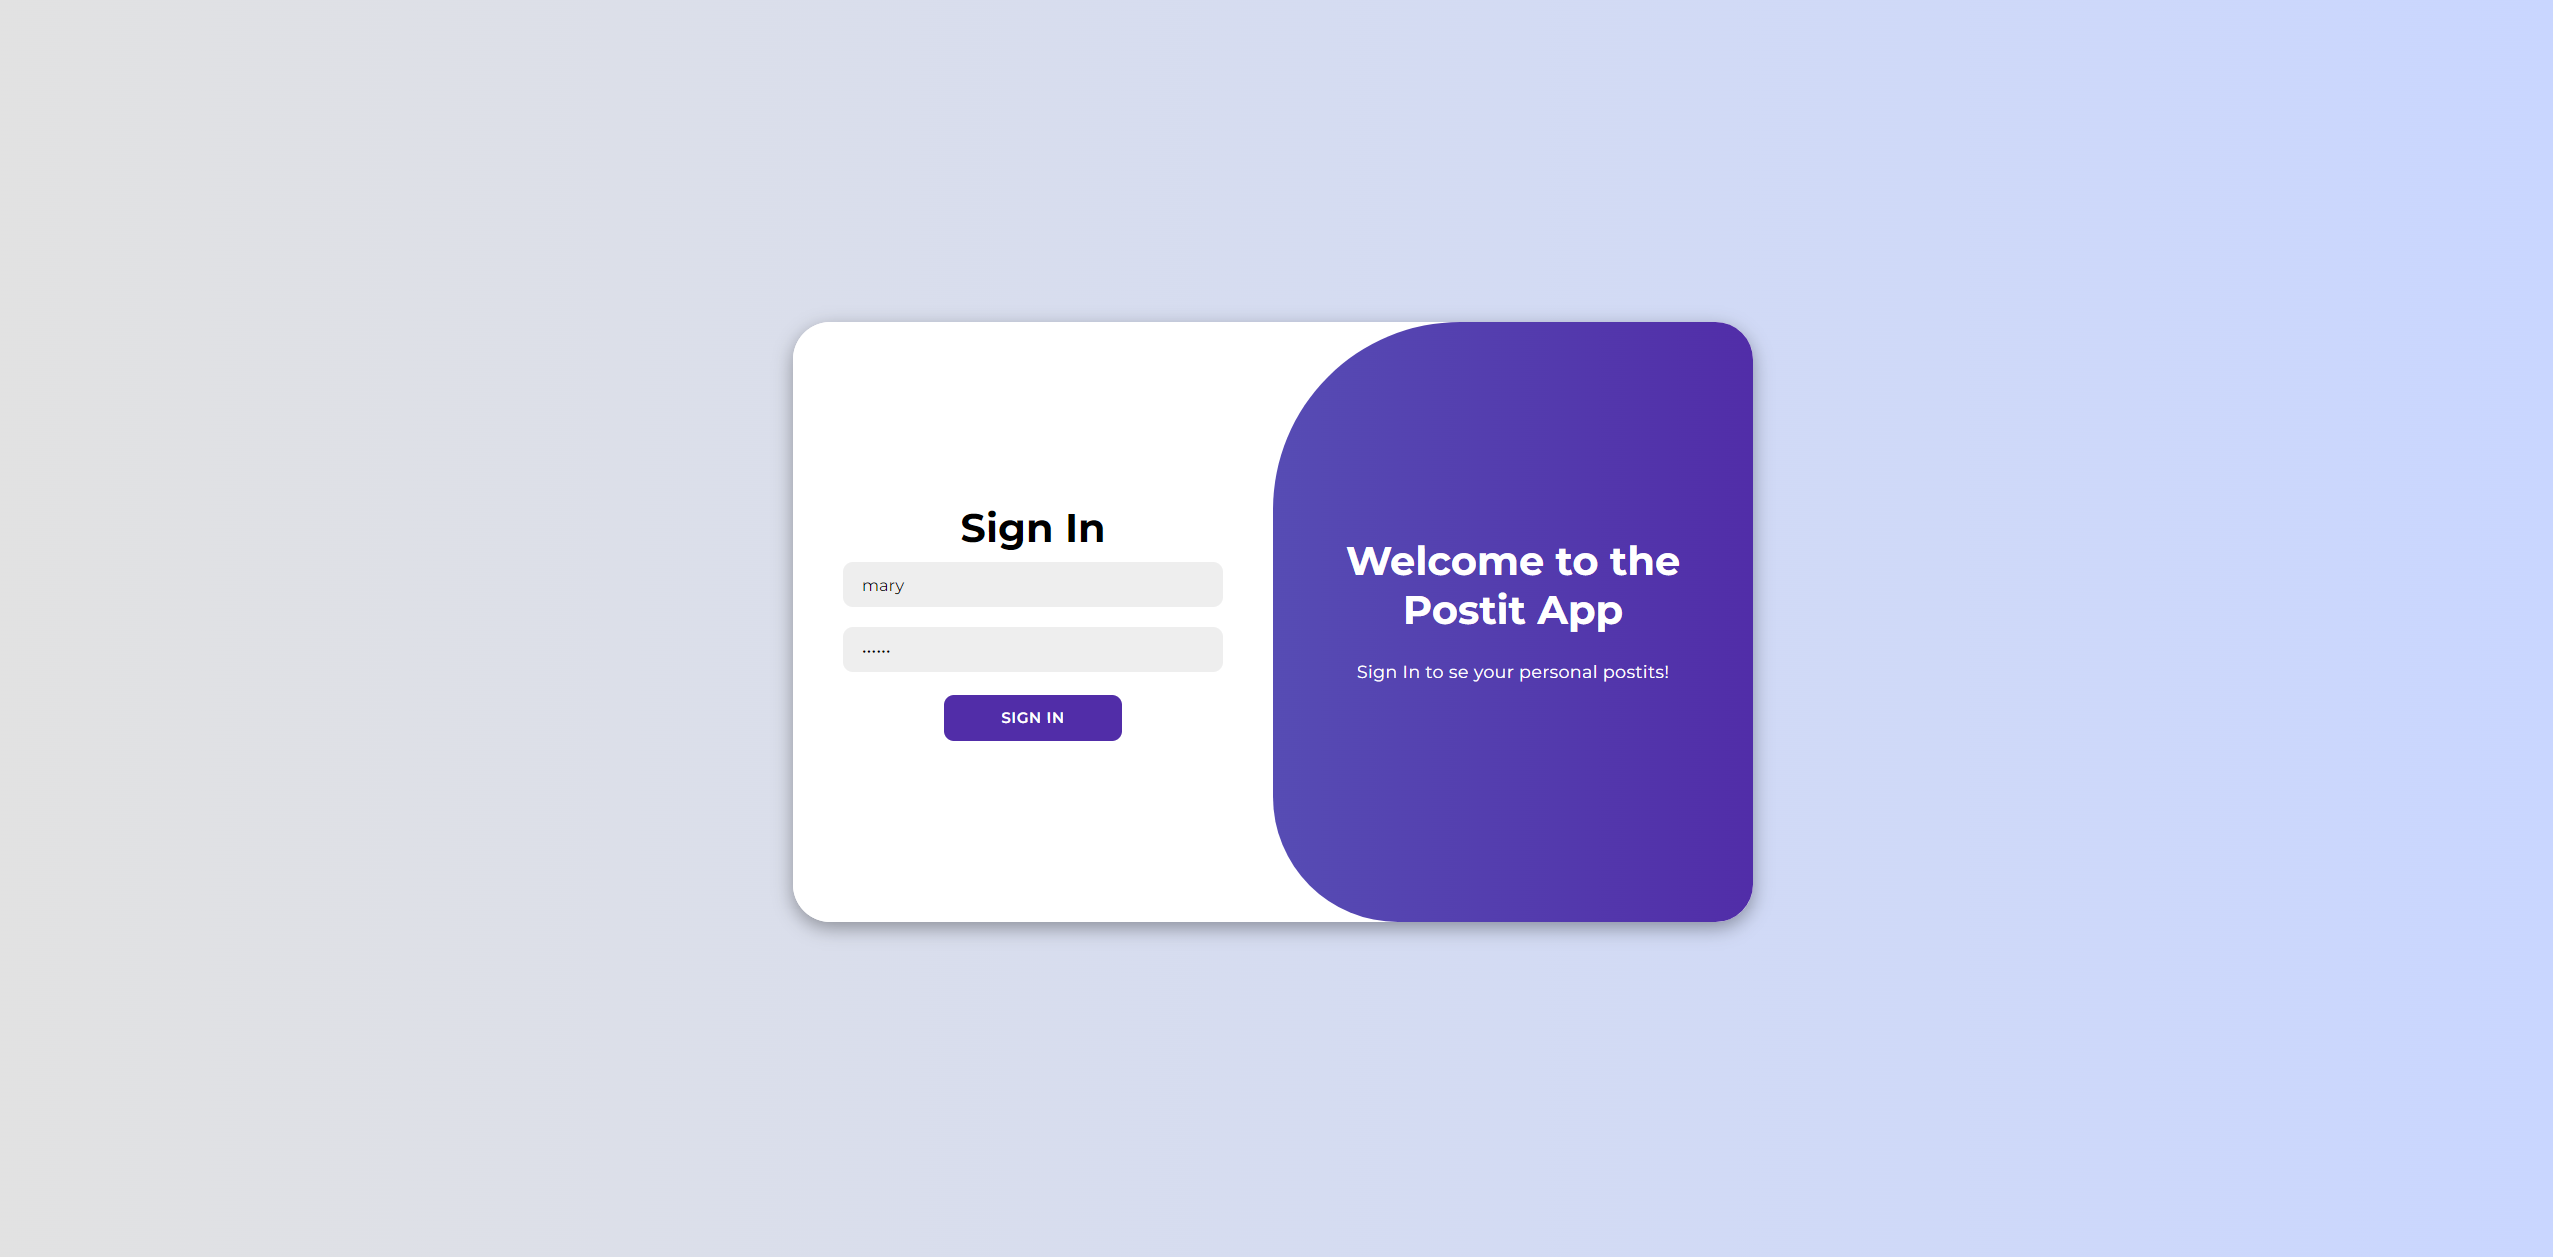
\includegraphics[width=0.9\textwidth]{images/1 login.png}
        \caption{Pagina di login}
         \subsubsection{Visualizza la homepage}
        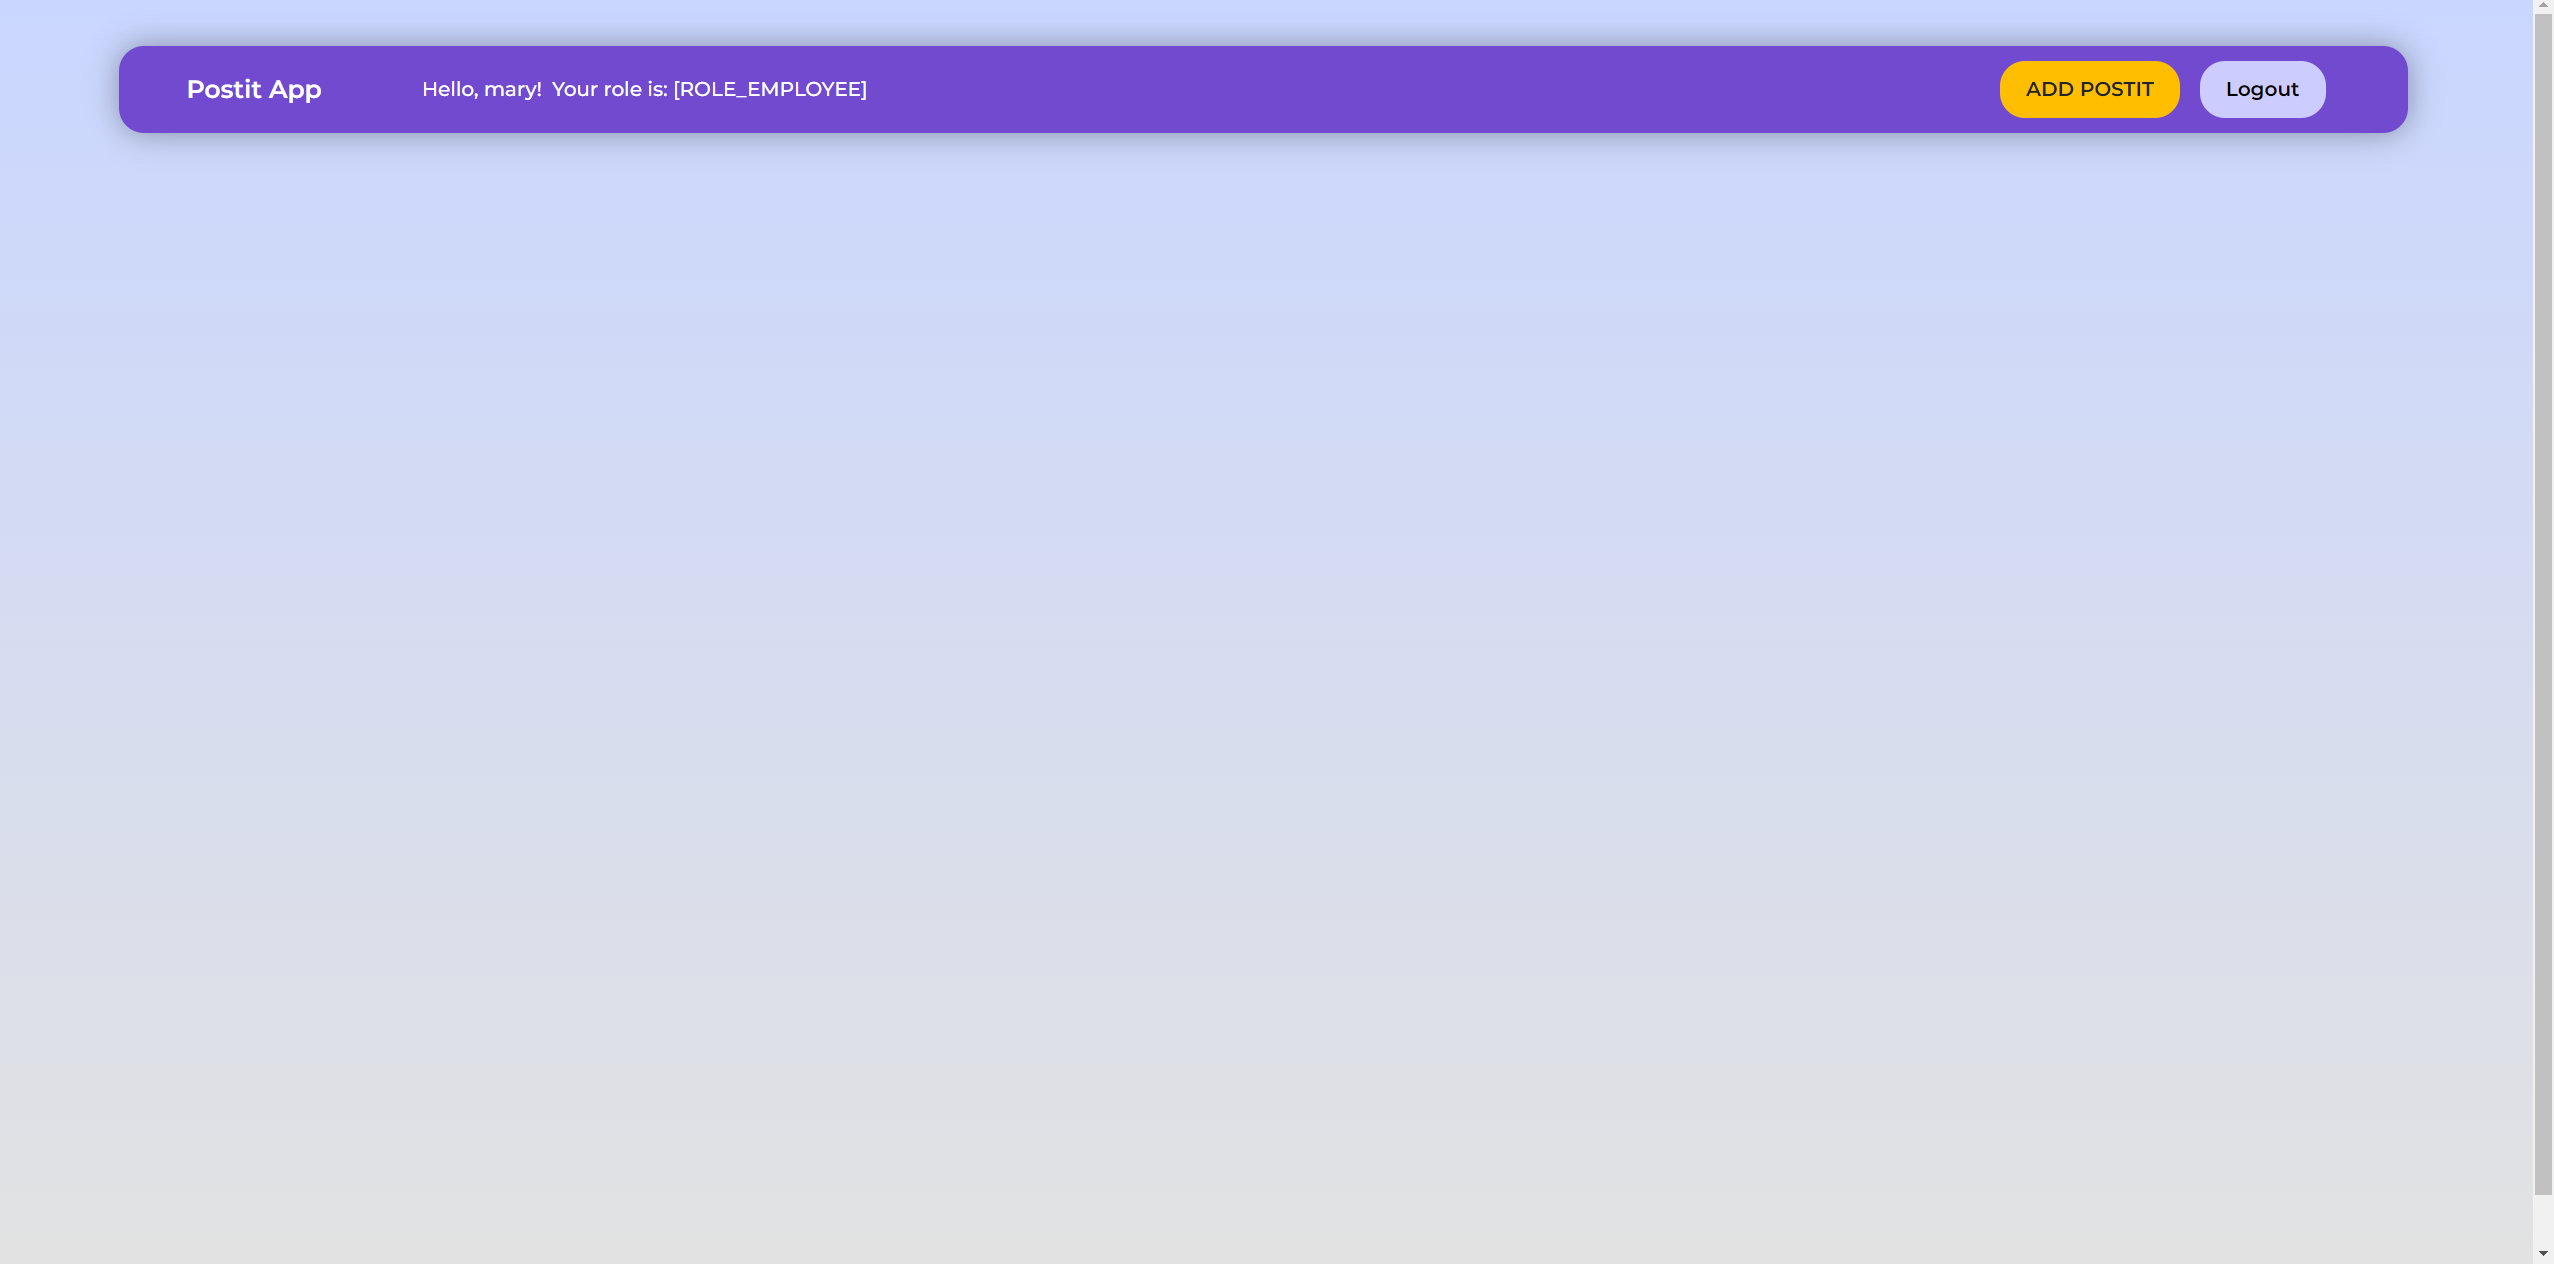
\includegraphics[width=0.9\textwidth]{images/2 homepage vuota.png}
        \caption{Home page}
        \label{fig:enter-label}
    \end{figure}
\end{center}
\vspace*{\fill}

\newpage

\vspace*{\fill}
\begin{center}
    \begin{figure}[h]
        \centering
        \subsubsection{Aggiunge 3 postit}
        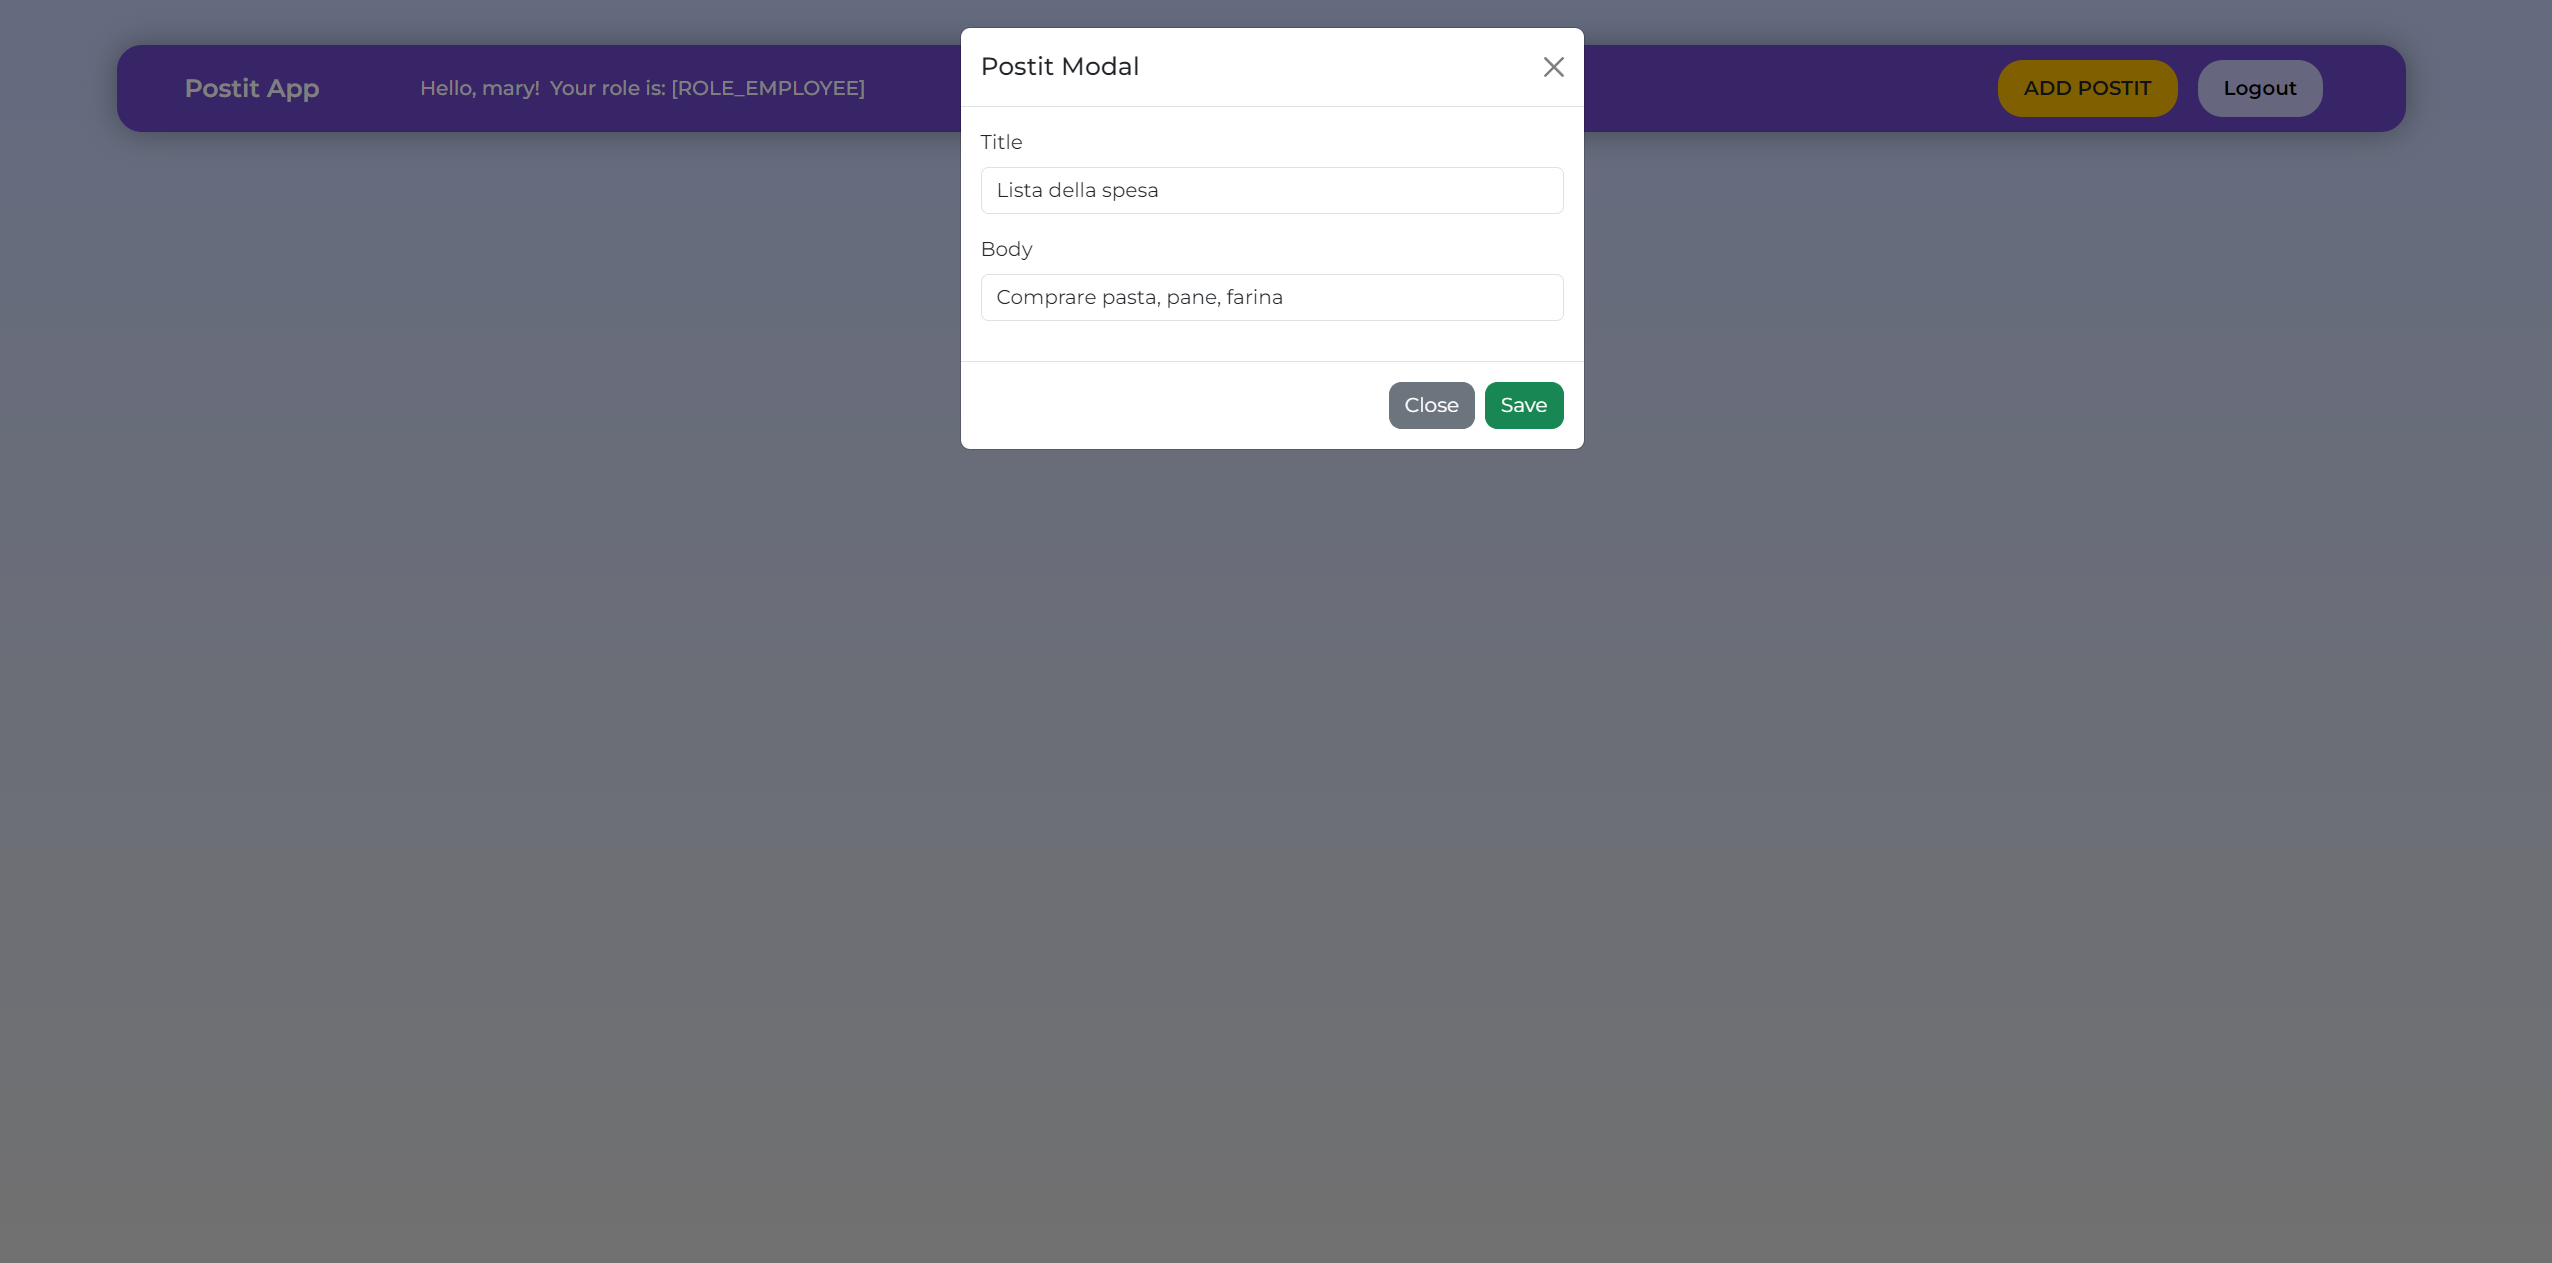
\includegraphics[width=0.9\textwidth]{images/3 aggiunta postit.png}
        \caption{Modal creazione postit}
         \subsubsection{Visualizza nella homepage i postit creati}
        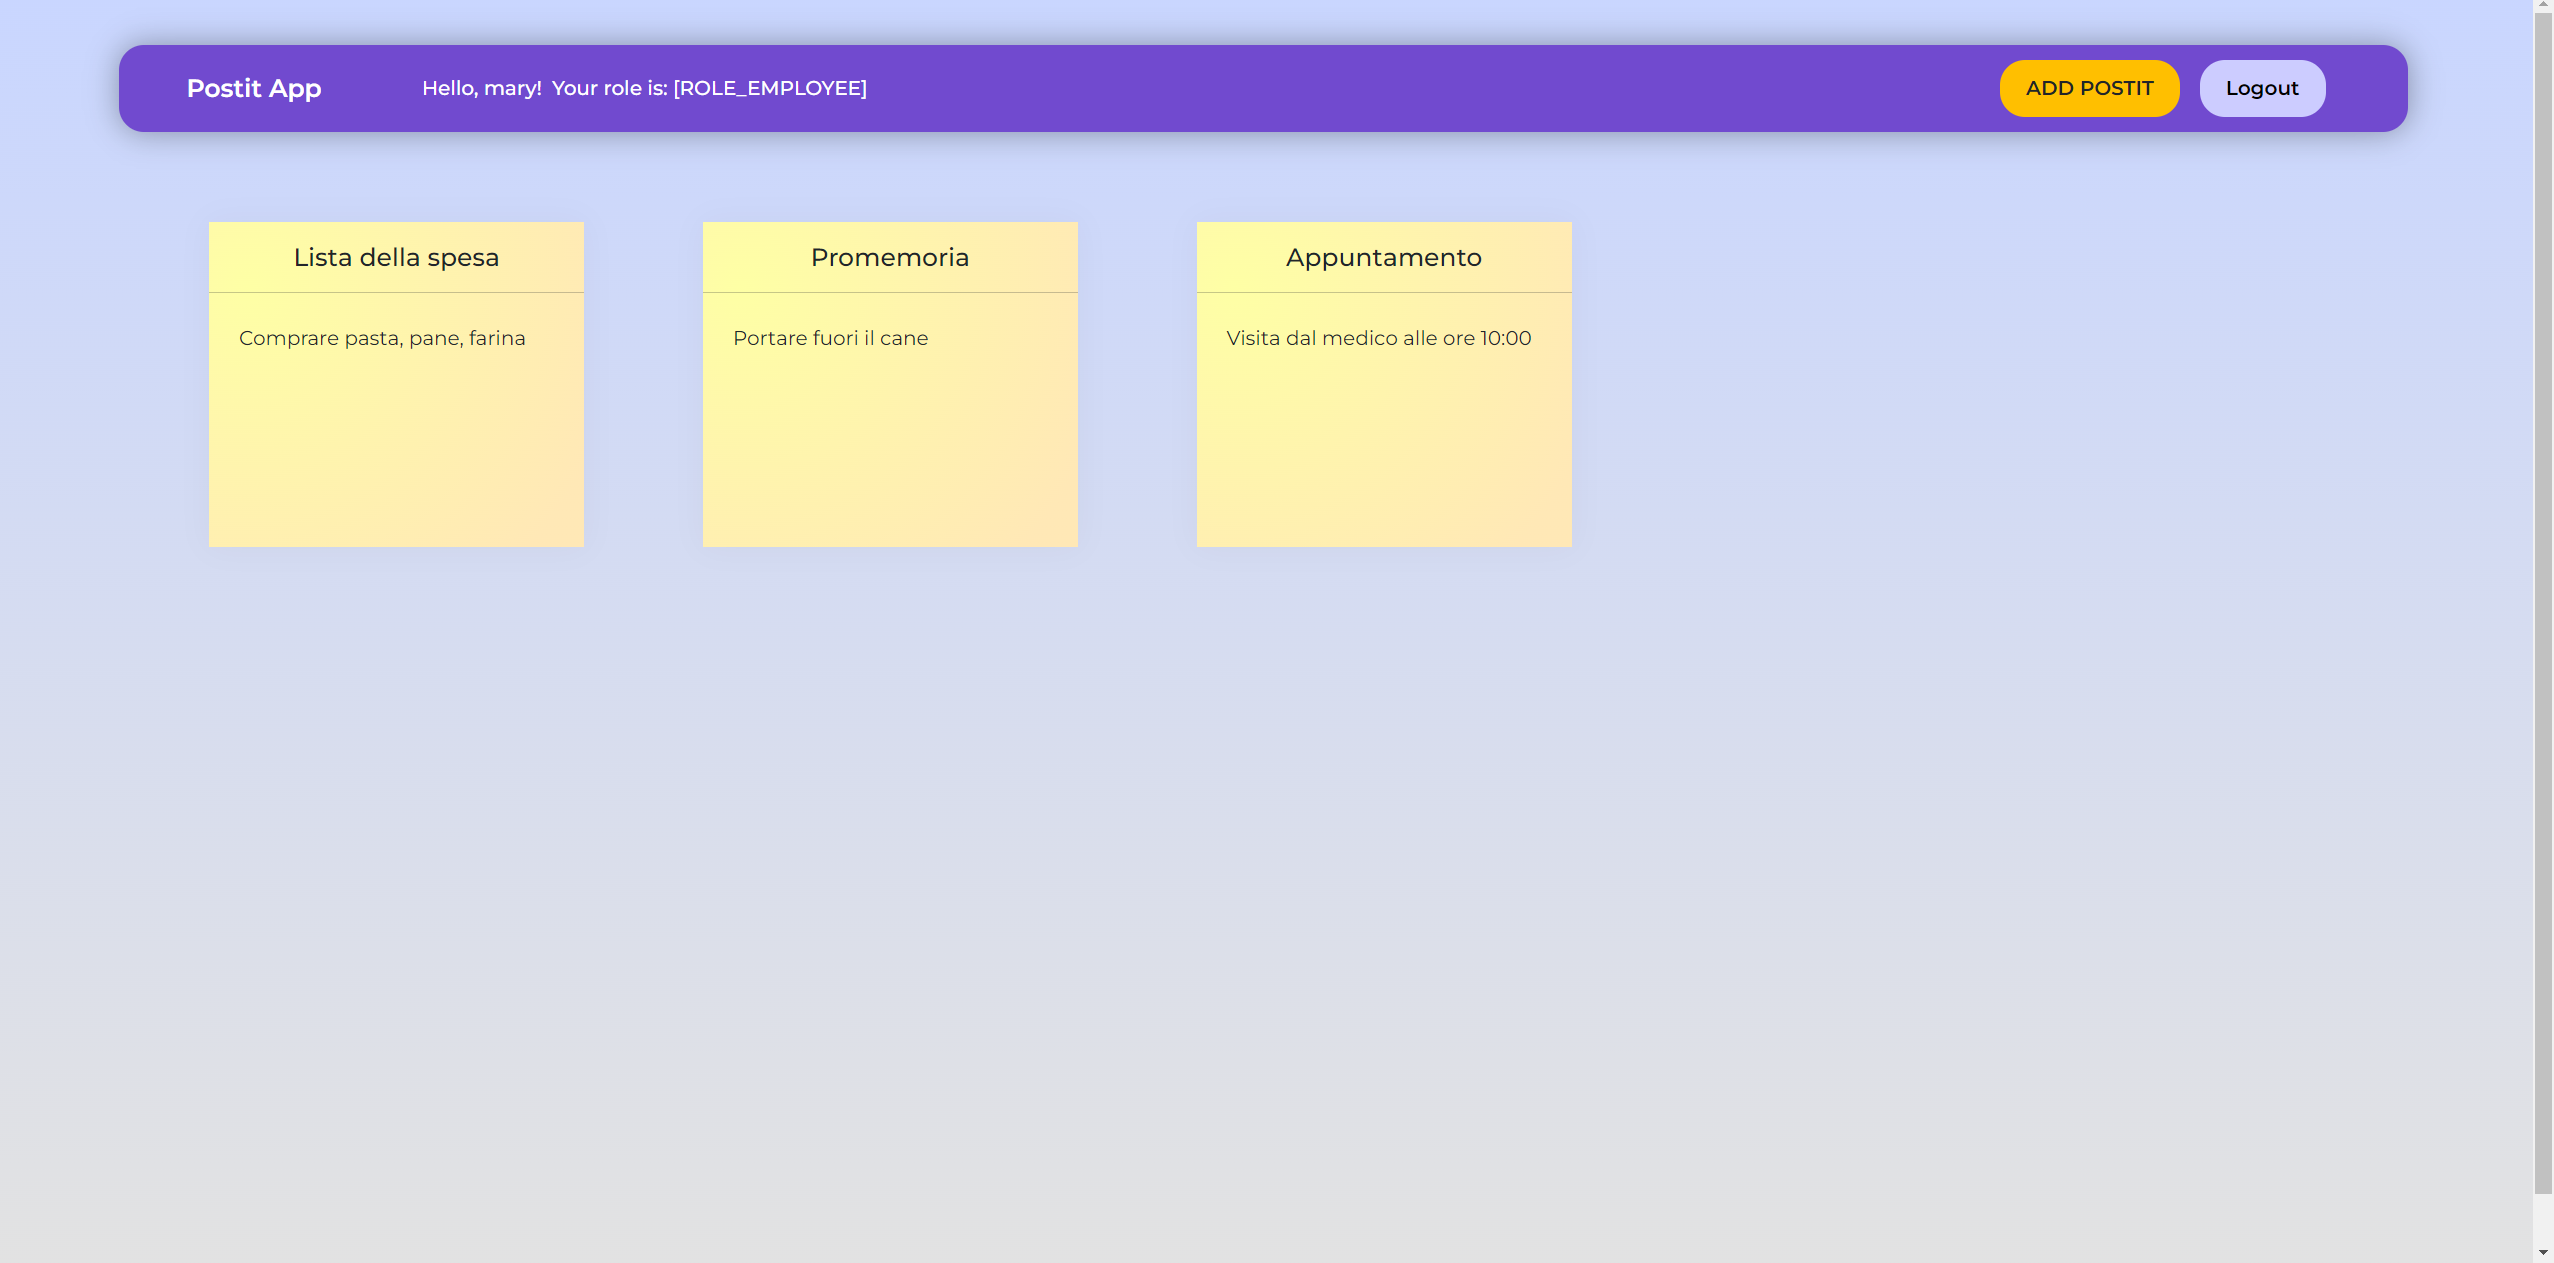
\includegraphics[width=0.9\textwidth]{images/4 postit visualizzati.png}
        \caption{Homepage che visualizza i 3 postit creati}
        \label{fig:enter-label}
    \end{figure}
\end{center}
\vspace*{\fill}

\newpage

\vspace*{\fill}
\begin{center}
    \begin{figure}[h]
        \centering
        \subsubsection{Modifica il primo postit}
        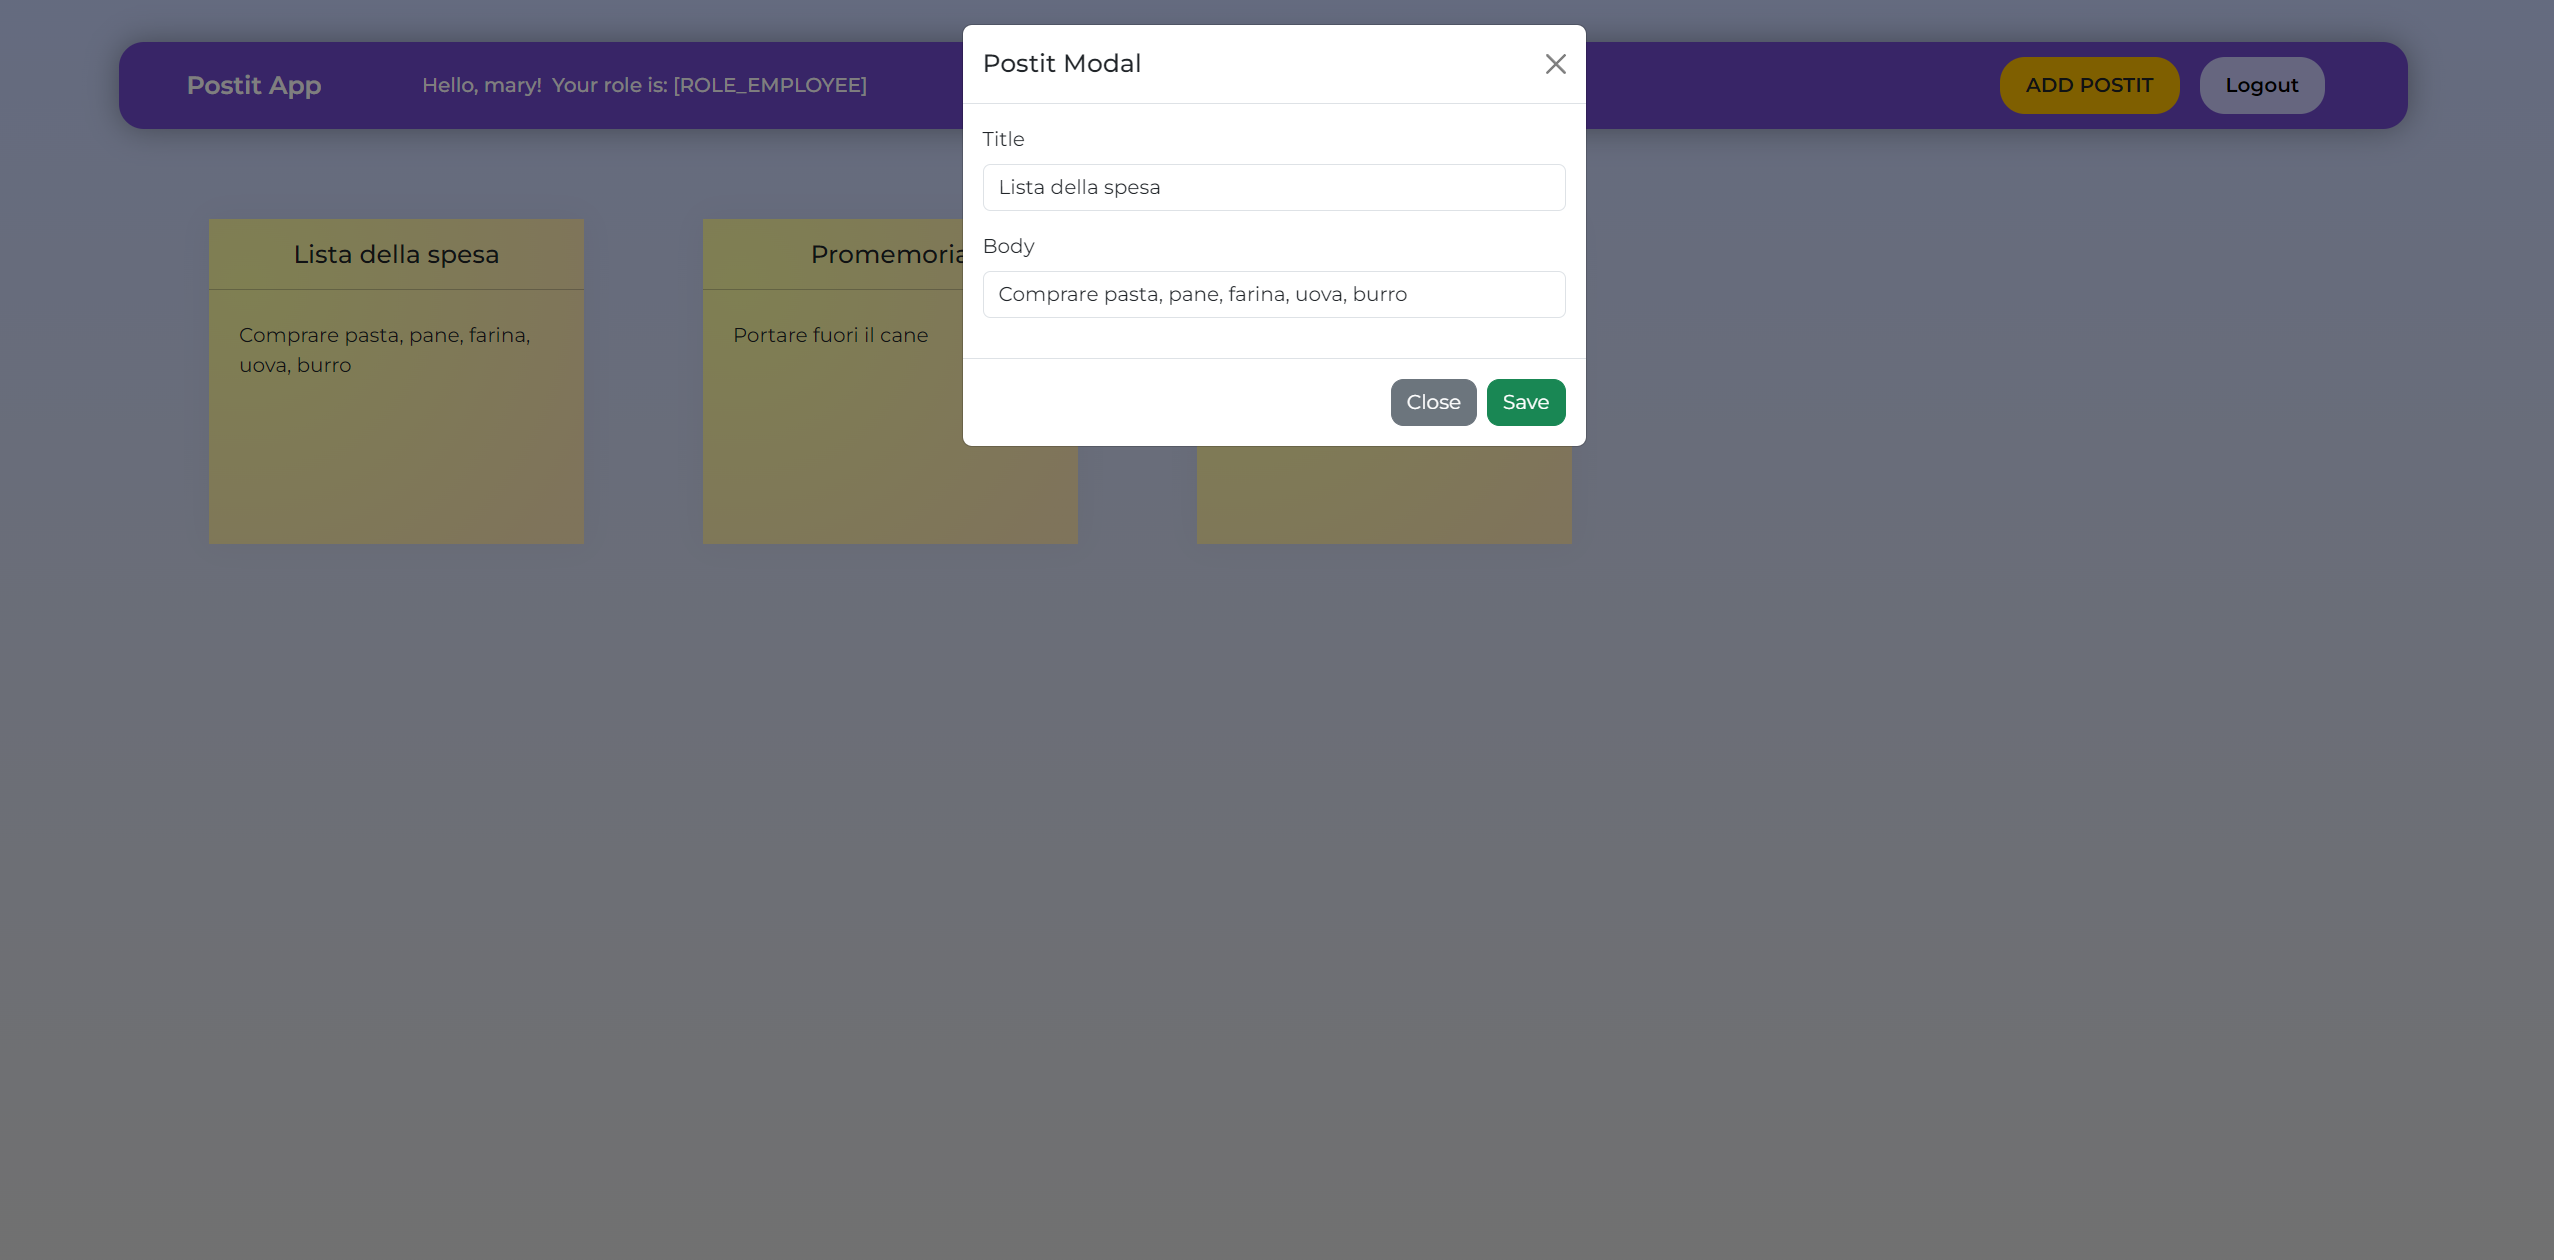
\includegraphics[width=0.9\textwidth]{images/5 modifica postit.png}
        \caption{Modal di modifica postit}
         \subsubsection{Elimina l'ultimo postit}
        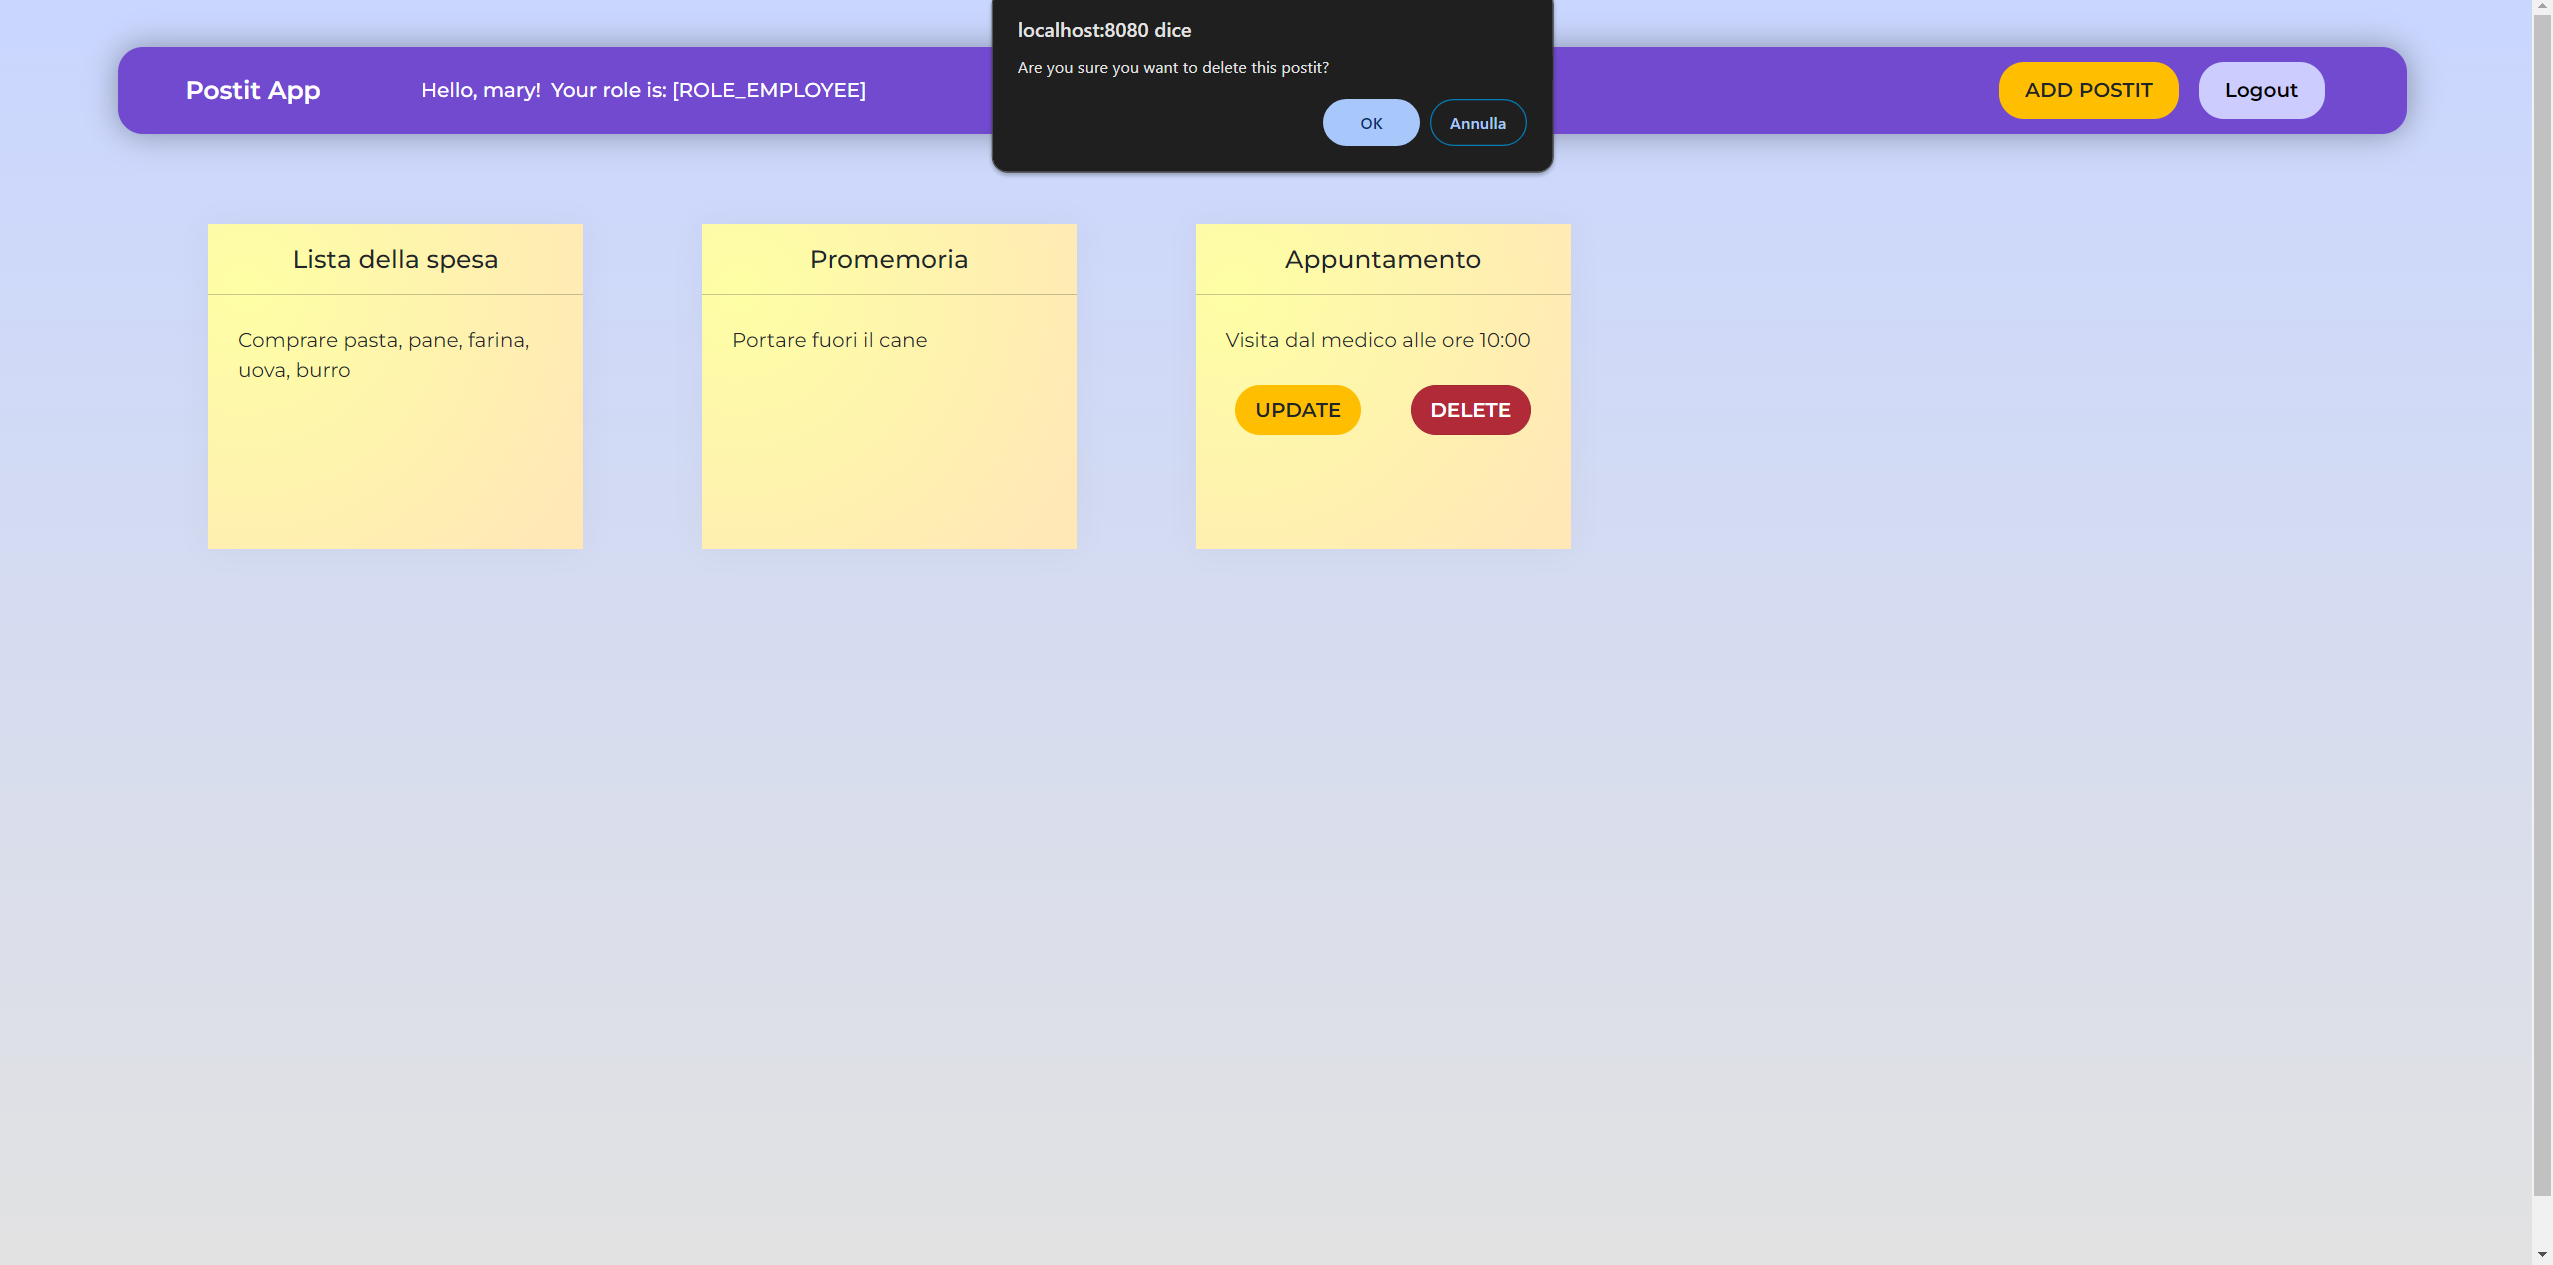
\includegraphics[width=0.9\textwidth]{images/6 eliminazione postit.png}
        \caption{Alert di eliminazione postit}
        \label{fig:enter-label}
    \end{figure}
\end{center}
\vspace*{\fill}

\newpage

\begin{center}
    \begin{figure}[th]
        \centering
        \subsubsection{Effettua il logout}
        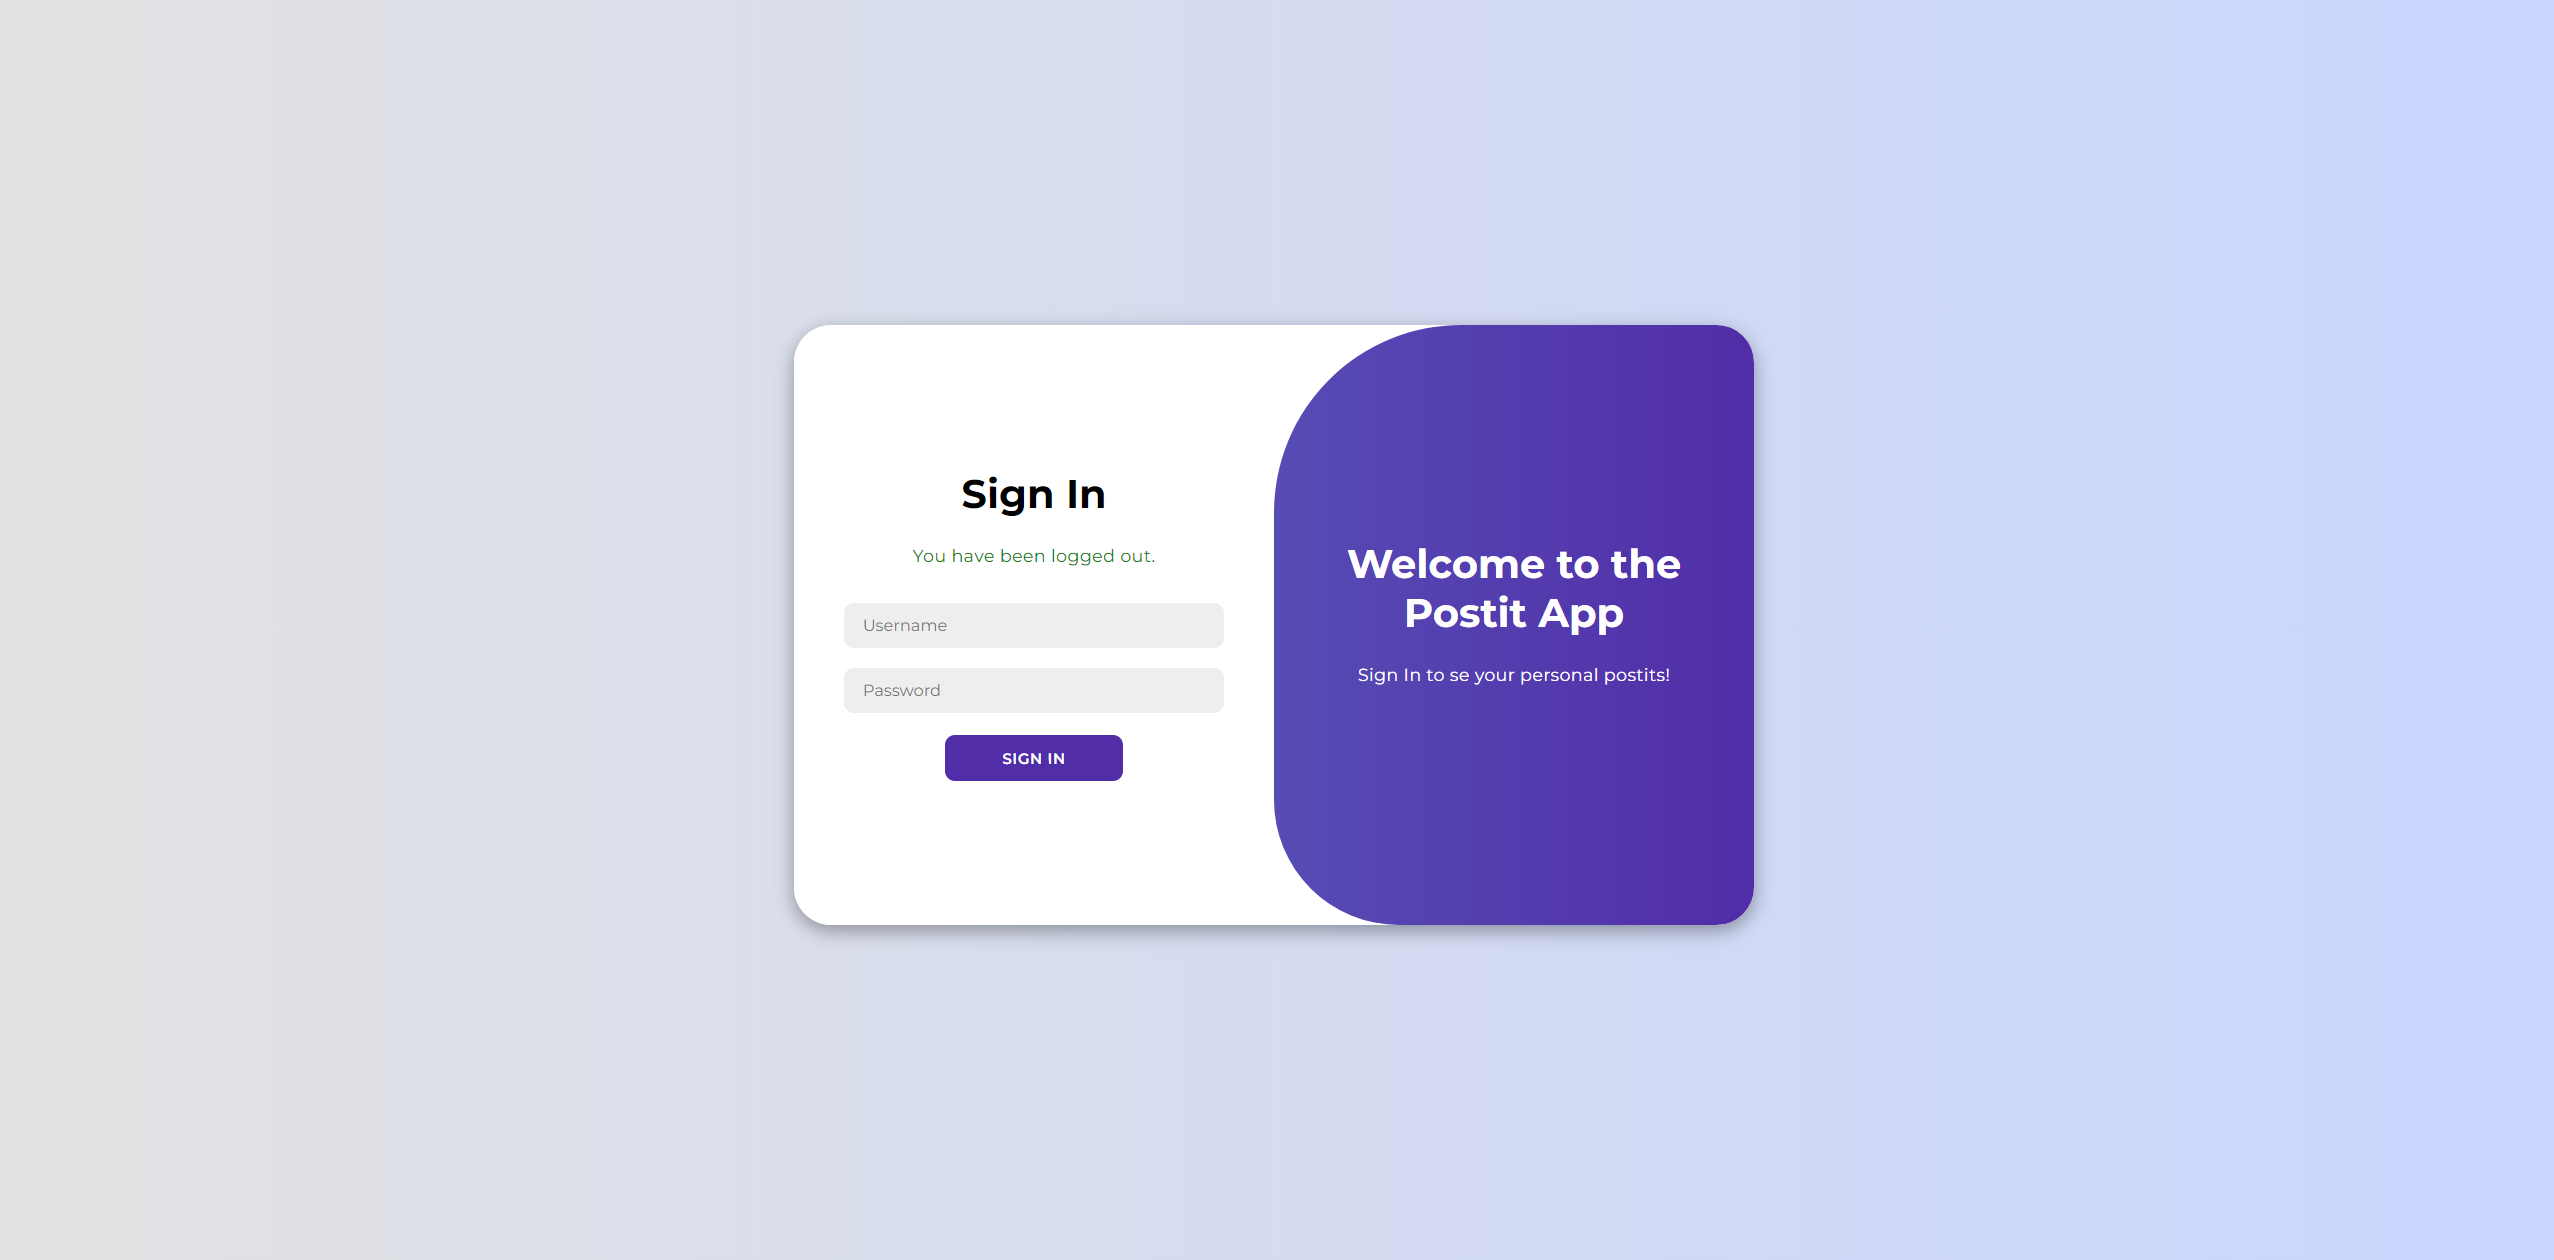
\includegraphics[width=0.9\textwidth]{images/7 logout.png}
        \caption{Pagina di login dopo aver effettuato il logout}
        \label{fig:enter-label}
    \end{figure}
\end{center}
\vspace*{\fill}
